% MATLAB Symbolic Math Tutorial
%  CS177 Individual Term Project 
%
%  Started by Mehreen Asad on 2011-04-23.
%
\documentclass[]{article}

% Use utf-8 encoding for foreign characters
\usepackage[utf8]{inputenc}

% Setup for fullpage use
\usepackage{fullpage}

% Uncomment some of the following if you use the features
%
% Running Headers and footers
%\usepackage{fancyhdr}

% Multipart figures
%\usepackage{subfigure}

% More symbols
\usepackage{amsmath}
\usepackage{amssymb}
\usepackage{latexsym}
\usepackage{hyperref}
\usepackage[all]{hypcap}
%\usepackage{graphicx}

% Surround parts of graphics with box
\usepackage{boxedminipage}

% Package for including code in the document
\usepackage{listings}

% If you want to generate a toc for each chapter (use with book)
\usepackage{minitoc}

% This is now the recommended way for checking for PDFLaTeX:
\usepackage{ifpdf}


\ifpdf
\usepackage[pdftex]{graphicx}
\else
\usepackage{graphicx}
\fi
\title{Term Project CS177 : Symbolic Integration using MATLAB Symbolic Math Toolbox}
\author{ Mehreen Asad }

\date{2011-05-04}

\begin{document}

\ifpdf
\DeclareGraphicsExtensions{.pdf, .jpg, .tif}
\else
\DeclareGraphicsExtensions{.eps, .jpg}
\fi

\maketitle


\begin{abstract}
This tutorial incorporates the basic concepts used in MATLAB Symbolic Math Toolbox with specific emphasis on Symbolic Integration. It starts by giving the basic concepts of Symbolic Operations and MATLAB Symbolic  Commands. The tutorial then introduces Symbolic Integration Concepts for both Indefinite and Definite Integration. To futher illustrate the concepts, four examples are provided with solutions to give the reader a full insight into the concept of Symbolic Integration in MATLAB. The tutorial is ideal for people who have never used MATLAB Symbolic Math Toolbox before.
\end{abstract}


\section{Symbolic Toolbox Basics}
\subsection{Concepts and Symbolic Matlab Commands}
\paragraph{}
Symbolic operations, like numerical operations can be performed by MATLAB when the Symbolic Math Toolbox is installed. Symbolic operations are carried out in the similar manner as numeric operations except for the fact that the former are performed on symbolic variables rather than numeric values. The Symbolic Math Toolbox Software can be used to perform mathematical operations and incorporates: \emph{Calculus}, \emph{Simplifications and Substitutions},   \emph{Variable-Precision Arithmetic}, \emph{Linear Algebra}, \emph{Solving Equations} and \emph{Integral Transforms and Z-Transforms}. The focus of this tutorial is on Symbolic Integration which is a part of Symbolic Calculus. First basic Symbolic concepts are introduced in the tutorial and then \emph{Symbolic Integration} is discussed in detail illustrated with sample problems and their solutions and graphs, starting with relatively simple examples and then moving on to a bit complex ones involving some of the MATLAB commands mentioned here in the tutorial.
 
\subsubsection{Creating a Symbolic Object}
\paragraph{}
Symbolic objects can be created using the \emph{sym} or \emph{syms} command. The command is of the form:

a=sym('a')
or 
sym a. 
\paragraph{}
The only difference between these two commands is that the object name is displayed in the first command. \emph{syms} is used to declare multiple symbolic objects at the same time.
Symbolic objects can be numbers as well as variables. If a number is declared as a symbolic object, then all calculations related to that symbolic number are carried out exactly with no numeric approximation. Consider the following example:

a=sym(3);
b=sym(8);
f=b/a+sqrt(2) gives the result:
\[
f=8/3+\sqrt2
\]
instead of any numerical value.
\subsubsection{Creating Symbolic Expressions}
\paragraph{}
A Symbolic Expression can be created by first defining symbolic objects and then writing an expression in terms of those symbolic objects. 
\paragraph{}
Using, the \emph{syms} command:
syms a b c x y
\[
f = ax^2+bxy+cy
\]
\subsubsection{Matlab Commands: }
\paragraph{}
The \emph{double(f)} command is used to transform a symbolic expression \emph{f} written in exact form to numerical form.
\paragraph{}
The \emph{collect(f)} Command groups the terms in the expression \emph {f} that have the variable with the same power.
\paragraph{}
The \emph{expand(f)} command expands expressions by carrying out products of terms that include summation and uses trigonometric identities and exponential and logarithmic laws to expand corresponding terms that include summation.
\paragraph{}
The \emph{factor(f)} command is the opposite of expand command and reduces the polynomial expression to be a product of polynomials of a lower degree.
\paragraph{}
The \emph{simplify(f)} and \emph{simple(f)} are used for simplifying the form of an expression. The command [F how] = simple(f) gives the simplified expression as well as the method used for simplifying the expression by assigning it to variable \emph{how}.
\paragraph{}
The \emph{pretty(f)} command displays a symbolic expression in a format resembling the mathematical format.
\paragraph{}
The \emph{findsym(f)} command displays the names of all symbolic variables in \emph{f} in alphabetical order.  
\paragraph{}
The \emph{solve(eq)} and \emph{solve(eq,var)} commands are used for solving the equation. The \emph{solve(eq)}  solves the equation for default variable \emph{x} and the \emph{solve(eq,var)} command can be used to solve the equation in terms of the variable \emph{var}. If there is only one variable, then the solution is numerical, otherwise the solution is in terms of other variables.

\section{Symbolic Integration Concepts}
\subsection{Concepts}
\paragraph{}
Symbolic Integration can be carried out by using the \emph{int} command. Both indefinite and definite Integrals are determined by the command \emph{int}. \emph{f} can be a pre-defined symbolic expression or an an expression can be typed in for \emph{f}
\subsection{Indefinite Integration}
\paragraph{}
If \emph{f} is a symbolic expression, the \emph{int(f)} attempts to find another symbolic expression \textbf{F} such that \emph{diff(F)}=\emph{f}.
\paragraph{}
If the expression contains one variable, then integration is carried out with respect to that variable using the \emph{int(f)} command.
\paragraph{}
If the expression contains more than one variable, then integration is carried out with respect to the desired variable using the \emph{int(f,var)} command.

\subsection{Definite Integration}
\paragraph{}
For definite Integration, the commands \emph{int(f,a,b)} and\emph{int(f,var,a,b)} are used for integration \emph{w.r.t} a particular variable. \textbf{a} and \textbf{b} are the limits of Integration. The limits can be \emph{inf} or \emph{-inf}.
\paragraph{}
In contast to differentiation, symbolic Integration is a more complicated task. The antiderivative \textbf{F} may not exist in closed form, or even if exists, MATLAB might not be able to find it. In case of such an exception, MATLAB returns \emph{int(f)} and a message \emph{Explicit Integral could not be found.}

%\subsection{Integration with real parameters}


\section{Symbolic Integration Examples}

\subsection{Example 1:  }
\subsubsection{Problem:}
\paragraph{}
Evaluate the indefinite Integral

\[
 I=\int\frac{sin^2(x)cos(x)}{(2+3sin(x))^2}dx.
\]
\paragraph{}
Display the result in mathematical format using \emph{pretty} command. Plot both the function and the Integral using subplot.
\subsubsection{Solution:}
\paragraph{}
The problem is solved by first declaring a symbolic variable x and then defining the function \emph{f} in terms of the symbolic variable. Then the Integral is computed using the \emph{int} command in Matlab. 
\DeclareGraphicsExtensions{.pdf,.png,.jpg}

The matlab commands are given in the project.m scipt file which contains solutions to all the problems mentioned in the tutorial.
\paragraph{}
Following are the plots for function and the Integral of Problem 1.
\paragraph{}

\begin{center}
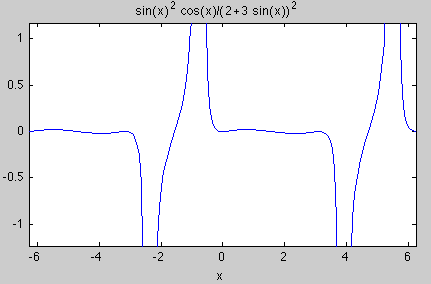
\includegraphics[width=8cm]{P1function}

\end{center}
\paragraph{}
\begin{center}
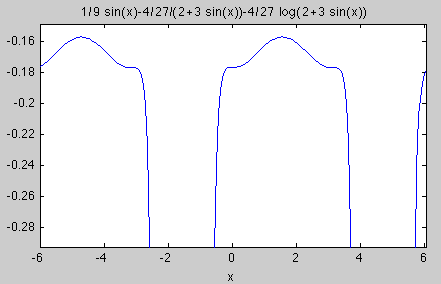
\includegraphics[width=8cm]{P1integral}
\end{center}

\subsection{Example 2:}
\subsubsection{Problem:}
\paragraph{}
The differential volume element of the cone is given by:
\[
dV=\pi(R^2)(1-\frac{y}{H})^2dy
%^3(1-\(frac{y}{H}^2)dy)
\]
\paragraph{}
Use MATLAB to evaluate the integral of dV from 0 to \emph{H} symbolically and show that the volume of the cone is 

\[
V=\frac{1}{3}\pi(R^3)H
\]



\subsubsection{Solution:}
\paragraph{}
The \emph{int} command is used to calculate the Integral for the given equation which gives the Volume \emph{V} of the cone.

\subsection{Example 3:  }
\subsubsection{Problem:}
\paragraph{}
The rms value of an AC Voltage is defined by:

\begin{equation} 
 v_{rms} = \sqrt{\frac{1}{T}\int_0^T v^2(t)\,dt}
\end{equation}


where T is the period of the waveform.
A voltage is given by
\[
 v(t) = Vcos(\omega t)
\]
Show that 
\[
v_{rms} = \frac{V}{\sqrt2} 
\]
and is independent of w.
Note: The relationship between the period \emph{T} and the radian frequency \emph{omega} is: 
\[
T = \frac{2\pi}{\omega}
\]

\subsubsection{Solution:}
First, the values of v(t) and T as given in the problem are substituted in Eq (1) and then the equation is being solved for 
\[
v_{rms} = \frac{V}{\sqrt2} 
\]
First symbolic variables are declared using \emph{syms} command:
syms T v V w t

Then, \emph{v(t)} and \emph{T} are defined in terms of symbolic variables. Next, eq(1) is solved in terms of V using the \emph{int} command for symbolic integration. The limits of integration are set from 0 to T. The solution is then further simplified by \emph{simple} command and [how] specifies the name of the simplification method.

\subsection{Example 4:  }
\subsubsection{Problem:}
\paragraph{}
A horizontal cylindrical tank is used for storing fuel. The tank has a diameter of 6 m and is 8 m long. The amount of fuel in the tank can be estimated by looking at the level of the fuel through a narrow vertical glass window at the front of the tank. A scale that is marked next to the window shows the level of the fuel corresponding to 40, 60, 80, 120, 160 thousand litres. Determine the vertical position (measured from the ground) of the lines of the scale. 
\paragraph{}
The volume \emph{V} of the fuel is given by:
\[
V=AL=L\int_0^h w\, dy
\]
where \emph{A} is the cross-sectional area of the fuel and \emph{L} is the length of the tank. The width \emph{w} of the top surface of the fuel is written as a function of \emph{y} and is given by:

\[
w=2\sqrt{R^2-(R-y)^2}
\] 
where \emph{R} is the radius of the tank.
\subsubsection{Solution:}
\paragraph{}
Here we have \emph{R} = 3 and \emph{L} =8. Then we declare \emph{w, y, h} as symbolic variables. Next, \emph{w} is written as a symbolic expression in terms of \emph{R} and \emph{y}. The Volume of the fuel at height \emph{h} can be calculated by substituting \emph{w} in the integral in the equation for the volume and carrying out the Integration using the \emph{int(S,y,0,h)} command where \emph{S} is the symbolic expression and is obtained by multiplying \emph{L} with \emph{w}. The result is an equation that gives the volume \emph{v} as a function of \emph{h}. The value of \emph{h} for a given \emph{V} is obtained by solving the equation for \emph{h} using the MATLAB command \emph{solve}. In the current scenario, the values of \emph{h} have to be determined for volumes of 40, 60, 80, 120 and 160 thousand litres. The solution is given in project.m script file.


\subsection{References:}
\paragraph{}
\href{http://en.wikipedia.org/wiki/Root_mean_square}{Web Reference for Problem 1}
\paragraph{}
\href{http://www.mathworks.com/help/toolbox/symbolic/}{Web Reference for Matlab Symbolic Math Toolbox Demos and Documentation}
\paragraph{}
MATLAB: An Introduction With Applications (Third Edition) by Amos Gilat
\bibliographystyle{plain}
\bibliography{}
\end{document}
